% algemene structuur:
%
% - wat is CHR?
% - CCHR: doelstellingen
% - taal
% - impl
% - bench


\documentclass{beamer}

\mode<article>
{
  \usepackage{fullpage}
  \usepackage{hyperref}
}

\mode<presentation>
{
  \usepackage{hyperref}
  \setbeamertemplate{background canvas}[vertical shading][bottom=white!10,top=blue!10]
  \usetheme{Warsaw}
%  \usefonttheme[onlysmall]{structurebold}
}

\usepackage{amsmath}
\usepackage{pst-tree}
\usepackage{pst-node}
\usepackage{pst-eps}
\usepackage{pstcol}
\usepackage{pstricks}
\usepackage{listings}
\usepackage{color}
\usepackage[dutch]{babel}
\usepackage{fancyvrb}
\usepackage{ulem}

\setbeamertemplate{example text}{Voorbeeld}
\renewcommand{\emph}[1]{\textit{{#1}}}
\definecolor{dgreen}{rgb}{0,0.7,0}
\definecolor{dbrown}{rgb}{0.4,0.3,0.1}
\newcommand{\bs}{$\backslash$}
\newcommand{\cConstr}[1]{\textcolor{blue}{#1}}
\newcommand{\cMacro}[1]{\textcolor{red}{#1}}
\newcommand{\cComment}[1]{\textcolor{dgreen}{#1}}
\newcommand{\cLogic}[1]{\textcolor{dbrown}{#1}}
\newcommand{\code}[1]{{\tt #1}}

\setbeamercolor{background canvas}{bg=white}
\setbeamertemplate{footline}[frame number]
%\setbeamertemplate{navigation symbols}{}

\title{CCHR: De snelste CHR implementatie}
\subtitle{Pieter Wuille}

\author{Promotor: \\
Prof. Dr. Bart Demoen \\
Begeleider: \\
Dr. ir. Tom Schrijvers}

\date{29 mei 2007}

\begin{document}

\frame{\titlepage}


\begin{frame}
  \frametitle{Overzicht}
  \tableofcontents
\end{frame}

\AtBeginSection[]
{
  \begin{frame}<beamer>
    \frametitle{Overzicht}
    \tableofcontents[current,currentsubsection]
  \end{frame}
}

\section{Inleiding}

\subsection{Wat is CHR?}

\begin{frame}[containsverbatim]
  \frametitle{CHR}
  \begin{block}{Wat is CHR?}
    \begin{itemize}
      \item Een hoog-niveau declaratieve taaluitbreiding (van hosttaal)
      \item Regelgebaseerde omzetting van CHR constraints naar \begin{itemize}
        \item Andere CHR constraints
        \item Built-in constraints (door hosttaal aangeboden)
      \end{itemize}
      \item In feite multiset herschrijfregels
    \end{itemize}
  \end{block}

\end{frame}

\subsection{Voorbeelden}

\begin{frame}[containsverbatim]
  \frametitle{CHR syntax}
  \begin{example}{Grootst gemene deler in CHR(Prolog)}
\begin{Verbatim}
:- chr_constraint prime(+int), upto(+natural).

upto(X) <=> X<2 | true.
upto(X) ==> X>1 | Y is X-1, upto(Y), prime(X).
prime(X) \ prime(Y) <=> Z is Y mod X, Z==0 | true.
\end{Verbatim}
  \end{example}

  \begin{block}{CHR Syntax}
    \begin{itemize}
      \item Regels voor herschrijven CHR constraint store
      \item Simplification, propagation en simpagation regels \begin{itemize}
        \item Simplification: {\em Rem} \code{<=>} {\em Guard} \code{|} {Body}
        \item Propagation: {\em Kept} \code{==>} {\em Guard} \code{|} {Body}
        \item Simpagation: {\em Kept} \bs {\em Rem} \code{<=>} {\em Guard} \code{|} {Body}
      \end{itemize}
    \end{itemize}
  \end{block}
\end{frame}

\subsection{Doelstellingen}

\begin{frame}
  \frametitle{CCHR}
  \begin{block}{CCHR}
    \begin{itemize}
      \item Een zo effici\"ent mogelijke CHR implementatie schrijven
      \item C als hosttaal gebruiken
    \end{itemize}
  \end{block}

  \begin{block}{Mogelijkheden C}
    \begin{itemize}
      \item Veel vrijheid datastructuren
      \item Directe geheugentoegang
      \item Bestaande optimaliserende compilers
    \end{itemize}
  \end{block}

\end{frame}

\section{De taal}

\subsection{Syntax}

\begin{frame}
  \frametitle{CCHR: De taal}
  \begin{block}{Syntax}
    \begin{itemize}
      \item Binnen een \code{cchr}-blok in C code
      \item Constraint declaraties (argumenten: meeste C types)
      \item Regels gelijkaardig aan CHR syntax
      \item Arbitraire C expressies en statements in guard en body
      \item Lokale variabelen in guard en body
      \item Logische variabelen zijn mogelijk
    \end{itemize}
  \end{block}
\end{frame}

\subsection{Voorbeelden}

\begin{frame}[containsverbatim]
  \frametitle{CCHR: Voorbeeld 1}
  \begin{example}[Voorbeeld 1]{\tiny
\begin{Verbatim}[commandchars=\\\{\}]
\cMacro{#include <stdio.h>}
\cMacro{#include <stdlib.h>}

\cMacro{#include "fib_cchr.h"} \cComment{/* header gegenereerd door CCHR compiler */}

cchr \{
  constraint \cConstr{fib}(int,long),\cConstr{init}(int);

  begin @ \cConstr{upto}(_) ==> \cConstr{fib}(0,1L), \cConstr{fib}(1,1L);
  calc @  \cConstr{upto}(Max), \cConstr{fib}(N2,M2) \bs \cConstr{fib}(N1,M1) <=> alt(N2==N1+1,N2-1==N1), N2<Max |
              \cConstr{fib}(N2+1, M1+M2);
\}

int main(int argc, char **argv) \{
  cchr_runtime_init();
  cchr_add_\cConstr{upto}_1(90); \cComment{/* voeg upto(90) toe */}
  cchr_consloop(j,\cConstr{fib}_2,\{
    printf("fib(%i,%li){\bs}n",cchr_consarg(j,\cConstr{fib}_2,1),(long)cchr_consarg(j,\cConstr{fib}_2,2));
  \});
  cchr_runtime_free();
  return 0;
\}
\end{Verbatim}
}  \end{example}
\end{frame}


\begin{frame}[containsverbatim]
  \frametitle{CCHR: Voorbeeld 2}
  \begin{example}[Voorbeeld 2]{\scriptsize
\begin{Verbatim}[commandchars=\\\{\}]
\cComment{/* definieer log_int_t als een logische variabele van int's */}
\cLogic{logical_header}(int,int,log_int_t)

\cComment{/* cchr blok */}
cchr \{
  constraint \cConstr{fib}(int,log_int_t)
          option(destr,\{\cLogic{log_int_t_destruct}($2);\})
          option(init,\{\cLogic{log_int_t_copy}($2);\});

  dup @ \cConstr{fib}(N,M1) \ \cConstr{fib}(N,M2) <=> \{ \cLogic{log_int_t_seteq}(M1,M2); \};
  f01 @ \cConstr{fib}(N,M) ==> N<2 | \{ \cLogic{log_int_t_setval}(M,1); \};
  fn  @ \cConstr{fib}(N,M) ==> N>1 |
    log_int_t M1=\cLogic{log_int_t_create}(), log_int_t M2=\cLogic{log_int_t_create}(),
    \cConstr{fib}(N-2,M1), \cConstr{fib}(N-1,M2),
    \{ \cLogic{log_int_t_setval}(M,\cLogic{log_int_t_getval}(M1)+\cLogic{log_int_t_getval}(M2)); \},
    \{ \cLogic{log_int_t_destruct}(M1); \cLogic{log_int_t_destruct}(M2); \};
\}
\end{Verbatim}
}
  \end{example}
\end{frame}

\section{Implementatie}

\subsection{Overzicht}

\begin{frame}[containsverbatim]
  \frametitle{Opbouw CCHR}
  \begin{columns}[c]
  \column{0.40\textwidth}
  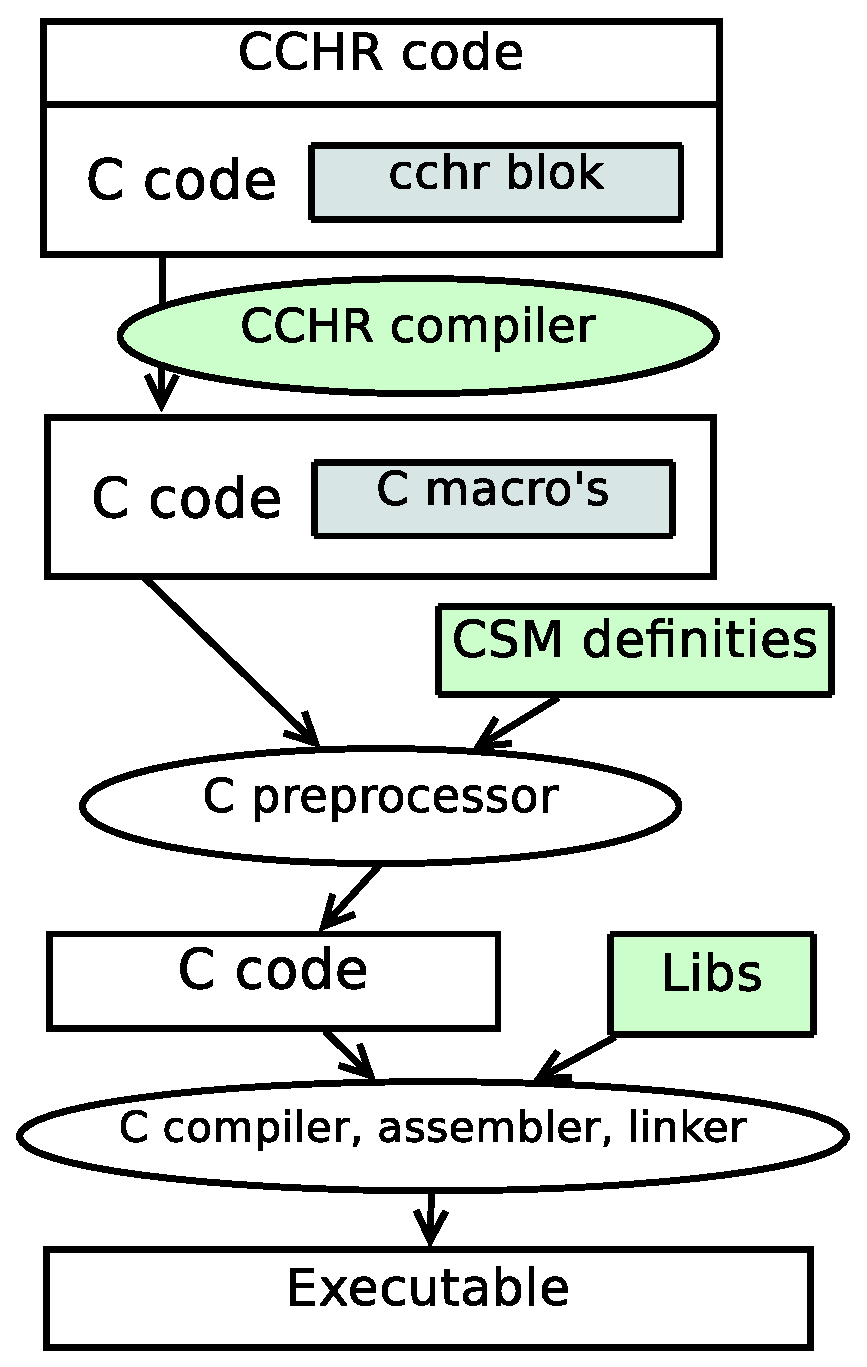
\includegraphics[height=0.83\textheight]{fig/overzicht}
  \column{0.60\textwidth}
  \begin{block}{Compilatieproces}
    \begin{itemize}
      \item CCHR code wordt door CCHR compiler doorlopen
      \item C code kopi\"eren, CCHR code vertalen naar macro's
      \item Gegenereerde code compileren (mbv. CSM definities)
      \item Extra libs (bv. code voor hashtable) compileren
      \item Samen linken tot executable
    \end{itemize}
    Het resultaat is een platform-specifiek, effici\"ent programma.
  \end{block}
  \end{columns}
\end{frame}

\subsection{CCHR Compiler}

\begin{frame}
  \frametitle{CCHR Compiler}
  \begin{block}{Componenten compiler}
    \begin{enumerate}
      \item Main routine: C code kopi\"eren en CCHR blokken detecteren
      \item Lexen van CCHR blok
      \item Parsen van CCHR blok, opbouwen AST
      \item Converteren van AST naar semantic tree
      \item Analyseren ST
      \item Berekenen goede ``join ordering''
      \item Genereren C macro's
      \item Uitvoermodule
    \end{enumerate}
  \end{block}
\end{frame}

\begin{frame}
  \frametitle{Implementatie CCHR Compiler}
  \begin{block}{Implementatie CCHR Compiler}
    \begin{itemize}
      \item De lexer is geschreven mbv. Flex
      \item De parser is geschreven mbv. Bison
      \item De rest van de compiler is in C geschreven
    \end{itemize}
  \end{block}
% eventueel iets over scheiding modules of efficientie
\end{frame}

\subsection{Gegenereerde code}

\begin{frame}
  \frametitle{
      
\end{document}

